\section{Sampling the System}
discuss the importance of sampling the system. When sampling the system, the correct time-delta must be selected which depends on the highest frequency which occurs in a time-reactive function in the whole system. For example in the FrSIR model we want infected agents to make on average contact with 5 other agents per time-unit, which means with a frequency of $frac{1}{5}$. This functionality is built on Yampas function occasionally which behaviour we investigated under differing time-deltas with the above frequency. In this investigation we simply sampled occasionally with different time-deltas for a duration of 1000 time-units and the event-frequency of $frac{1}{5}$. The results can be seen in Figure \ref{fig:sampling_occasionally_5evts} and are quite striking. The plot clearly shows that occasionally needs quite high sampling frequency even for comparatively low event-frequency - this becomes of course worse for higher event-frequencies.

\begin{figure}
	\centering
	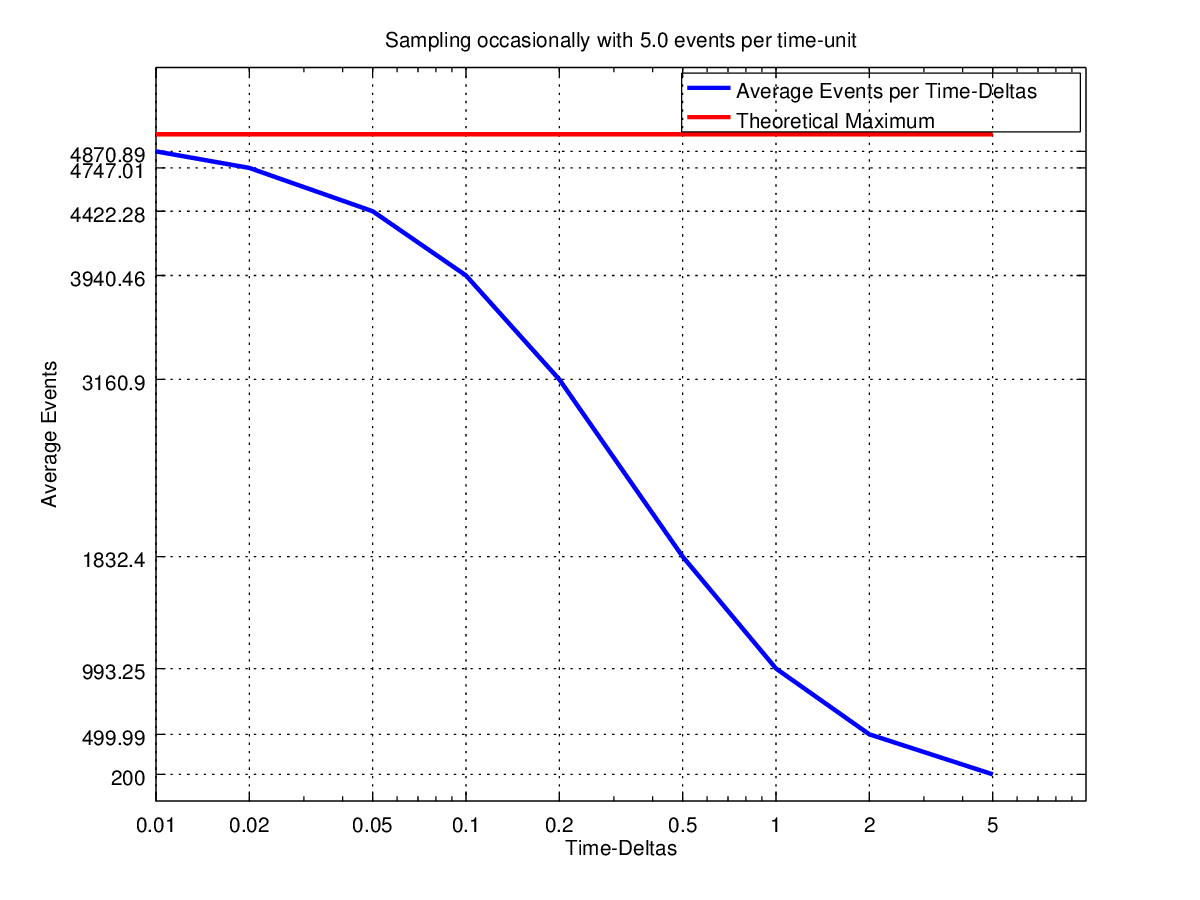
\includegraphics[width=.6\textwidth, angle=0]{./../shared/fig/samplingTest_occasionally_5evts.png}
	\caption{Sampling the \textit{occasional} function to visualize the influence of sampling frequencies on the event occurrence. Event-frequency of $\frac{1}{5}$ (average of 5 events per time-unit) with time-deltas of [ 5, 2, 1, $\frac{1}{2}$, $\frac{1}{5}$, $\frac{1}{10}$, $\frac{1}{20}$, $\frac{1}{50}$, $\frac{1}{100}$ ] running for 1000 time-units with 100 replications. The theoretical average is 5000 events within this time-frame.}
	\label{fig:sampling_occasionally_5evts}
\end{figure}

The other time-reactive function which occurs in the FrSIR model is the timed transition from infected to recovered which occurs on average with an exponential random-distribution after 15 time-units. This functionality is built on a custom implementation of Yampas after which creates an event after a time-out of the passed in time-duration drawn from an exponential random-distribution. Clearly this function has different semantics as although it also continuously emit events over time - NoEvent before the time was hit, and Event x after the time hit - the relevant point is that it switches to Event at some discrete point in time. This is implemented as simply adding up the time-deltas until the accumulator is GE than the previously drawn exponential time-out. We also investigated the behaviour of this function under varying time-deltas using a time-out of 15 (drawn from an exponential distribution within the function). Our approach was to sample the afterExp until an event occurs (this is one of the occasions where lazy evaluation really shines as one simply repeats the time-delta stream forever but then searches for the first occurrence of an event, which MUST occur at some point due to mathematical exponential distribution and our parameters to it, so it will always terminate) and then see when it has occurred. We run this with 10,000 replications with different random-number seeds and average the resulting times. The results can be seen in Figure \ref{fig:sampling_afterExp_5time}. The result is striking in another way: this function seems to be pretty invariant to the time-deltas, for obvious reasons: we are basically just interested in the "after"-condition of the whole semantics whereas in occasionally we are interested in the "repeatedly"-conditions. If we under the afterExp then we can be off by one time-delta. If we under sample occasionally we keep loosing events, the close time-delta and event-frequency are, the more we lose. Of course afterExp can also be used for very short time-outs e.g. $frac{1}{5}$. We have investigated the behaviour of this function for various time-deltas as well as seen in Figure \ref{sampling_occasionally_02evts}. Here the result is much more striking and shows that afterExp is vulnerable to small time-outs as well as occasionally. 
To show that occasionally is not vulnerable to very low frequencies of e.g. one event every 5 time-steps we plotted the behaviour of this under varying time-steps in Figure \ref{fig:sampling_occasionally_02evts}. The result shows that for low frequencies occasionally works fine with larger time-deltas

\begin{figure}
	\centering
	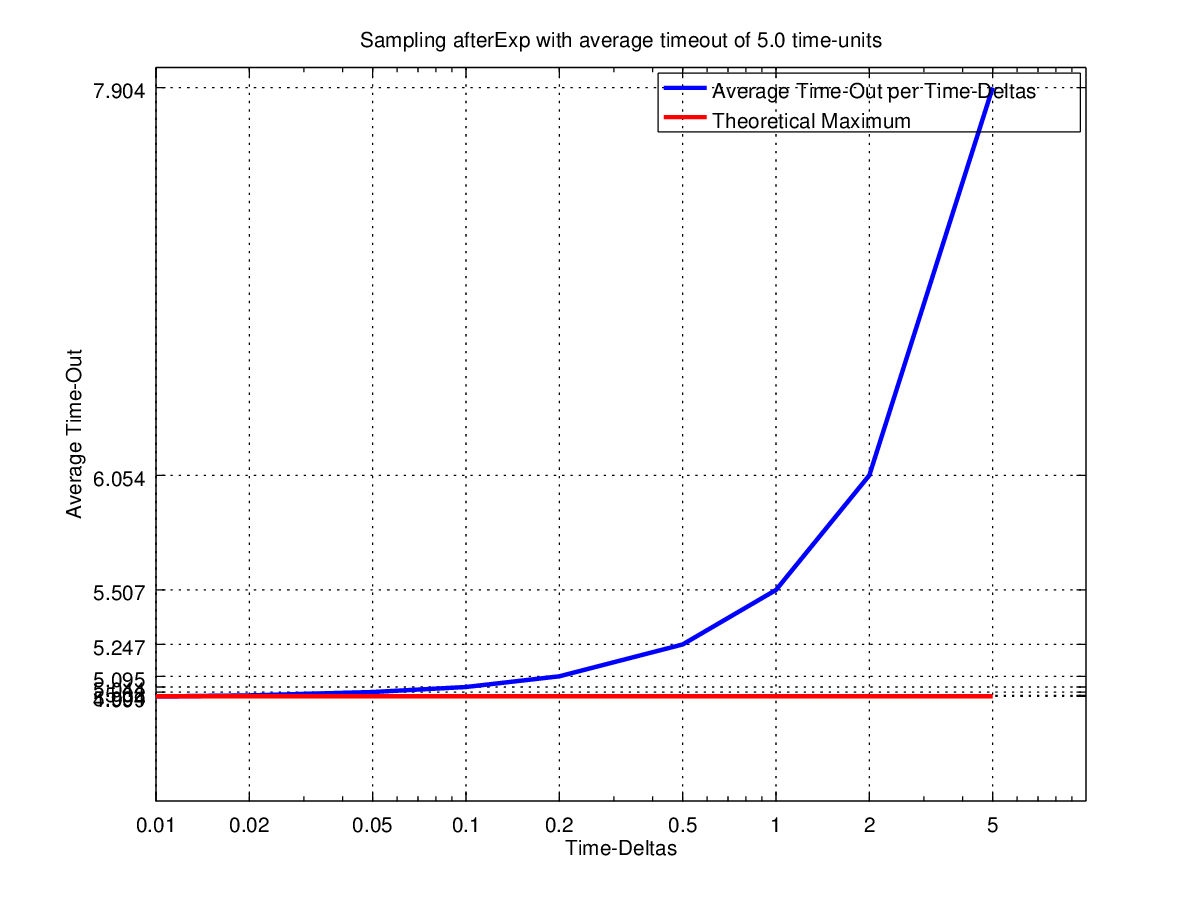
\includegraphics[width=.6\textwidth, angle=0]{./../shared/fig/samplingTest_afterExp_5time.png}
	\caption{Sampling the \textit{afterExp} function to visualize the influence of sampling frequencies on the occurrence of the time-out event. Average time-out of 5 with time-deltas of [ 5, 2, 1, $\frac{1}{2}$, $\frac{1}{5}$, $\frac{1}{10}$, $\frac{1}{20}$, $\frac{1}{50}$, $\frac{1}{100}$ ] running 10,000 replications.}
	\label{fig:sampling_afterExp_5time}
\end{figure}

\begin{figure}
	\centering
	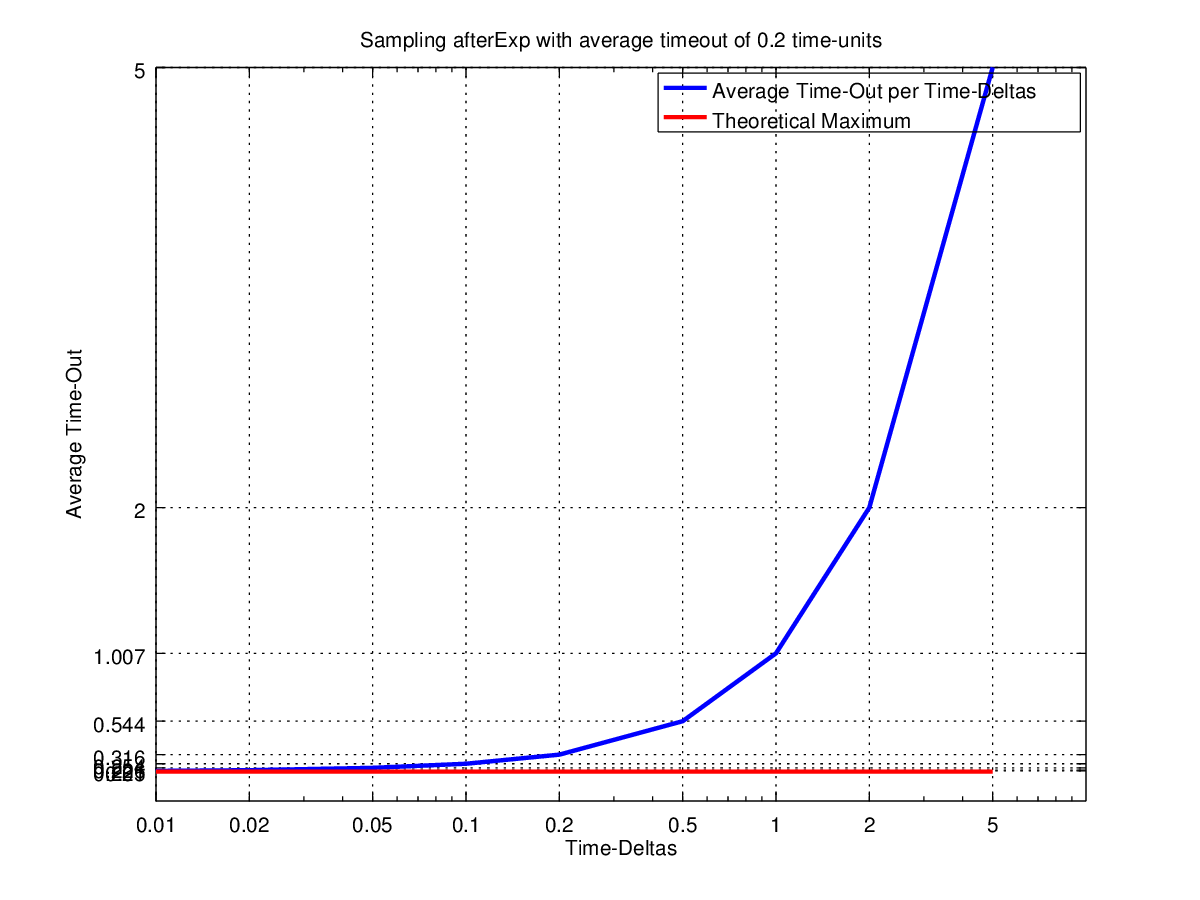
\includegraphics[width=.6\textwidth, angle=0]{./../shared/fig/samplingTest_afterExp_02time.png}
	\caption{Sampling the \textit{afterExp} function to visualize the influence of sampling frequencies on the occurrence of the event. Average time-out of 0.2 with time-deltas of [ 5, 2, 1, $\frac{1}{2}$, $\frac{1}{5}$, $\frac{1}{10}$, $\frac{1}{20}$, $\frac{1}{50}$, $\frac{1}{100}$ ] running 10,000 replications.}
	\label{fig:sampling_afterExp_02time}
\end{figure}

\begin{figure}
	\centering
	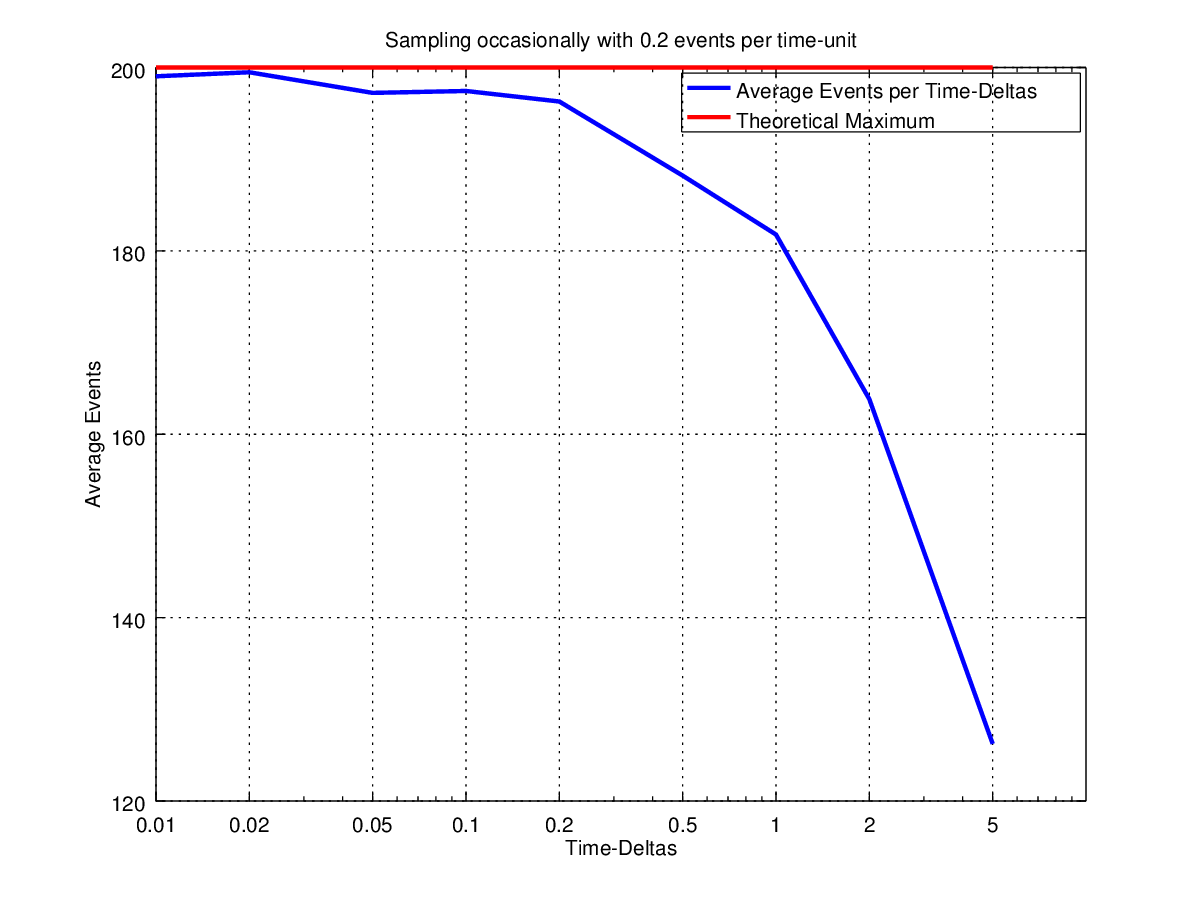
\includegraphics[width=.6\textwidth, angle=0]{./../shared/fig/samplingTest_occasionally_02evts.png}
	\caption{Sampling the \textit{occasional} function to visualize the influence of sampling frequencies on the event occurrence. Event-frequency of 5 (average of 0.2 events per time-unit) with time-deltas of [ 5, 2, 1, $\frac{1}{2}$, $\frac{1}{5}$, $\frac{1}{10}$, $\frac{1}{20}$, $\frac{1}{50}$, $\frac{1}{100}$ ] running for 1000 time-units with 100 replications. The theoretical average is 200 event within this time-frame.}
	\label{fig:sampling_occasionally_02evts}
\end{figure}

\subsection{Frequency of an ABS}
TODO: can we derive a formula to calculate the optimal time-delta for a given agent-based model?

\subsection{Super-Sampling}
of course performance is a big issue and it decreases as time-deltas get smaller and smaller. if we could perform subsampling just for the given high-frequency function with the remaining system running in lower frequency then we could achieve substantial performance-increase.

formula of calculating-steps = steps per time-unit * time-to-run-the-simulation

The problem is that \textit{embed} does not really help because when running a sf with it, the signal-functions time does not advance. Thus we implemented a new signal-function which allows us to super-sample another signal-function.

\begin{minted}{haskell}
superSampling :: Int -> SF a b -> SF a [b]
\end{minted}

It takes the number of super-samples \textit{n} and the signal-function \textit{sf} to sample and returns a new signal-function which performs the super-sampling. It does this by evaluating sf for n times with dt of $\frac{dt}{n}$ and the same input argument a for all n evaluations. At time 0 no super-sampling is done and just a single output of sf is calculated. A list of b is returned with length of n containing the result of the n evaluations of sf. If 0 or less super samples are requested exactly one is calculated.

We ran tests super-sampling both \textit{occasionally} (Figure \ref{fig:sampling_occasionally_ss_02evts}, Figure \ref{fig:sampling_occasionally_ss_5evts}) and \textit{afterExp} (Figure ). They work the same way as above except that now the time-delta is fixed to 1.0 but using increasing numbers of super-samples. The results are as expected: as the number of super-samples increase, so increases the accuracy.

\begin{figure}
	\centering
	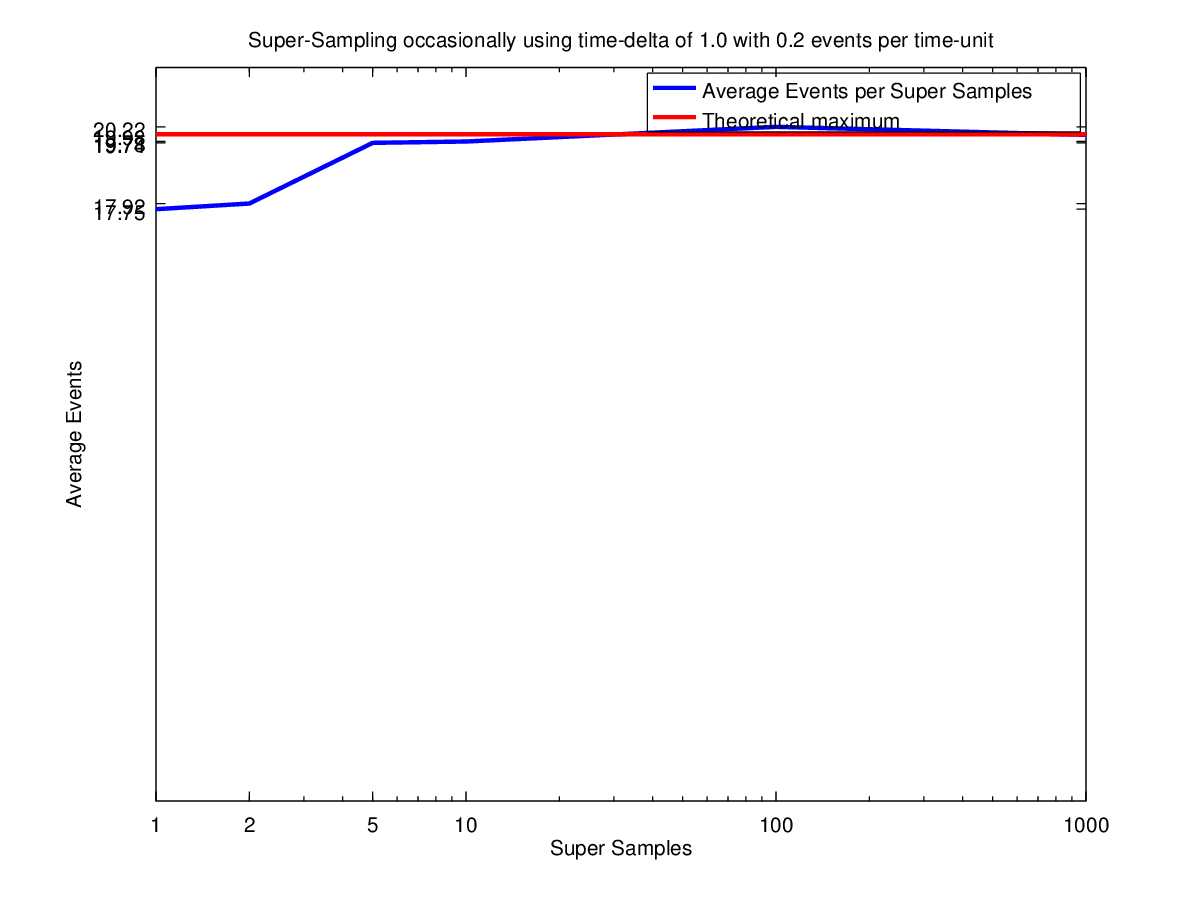
\includegraphics[width=.6\textwidth, angle=0]{./../shared/fig/samplingTest_occasionally_ss_02evts.png}
	\caption{Super-Sampling the \textit{occasional} function to visualize the influence of increasing number of super-samples on the event occurrence. Event-frequency of 5 (average of 0.2 events per time-unit) with time-delta of 1, with super-samples of [1, 2, 5, 10, 100, 1000] running for 100 time-units with 100 replications. The theoretical average is 20 event within this time-frame.}
	\label{fig:sampling_occasionally_ss_02evts}
\end{figure}

\begin{figure}
	\centering
	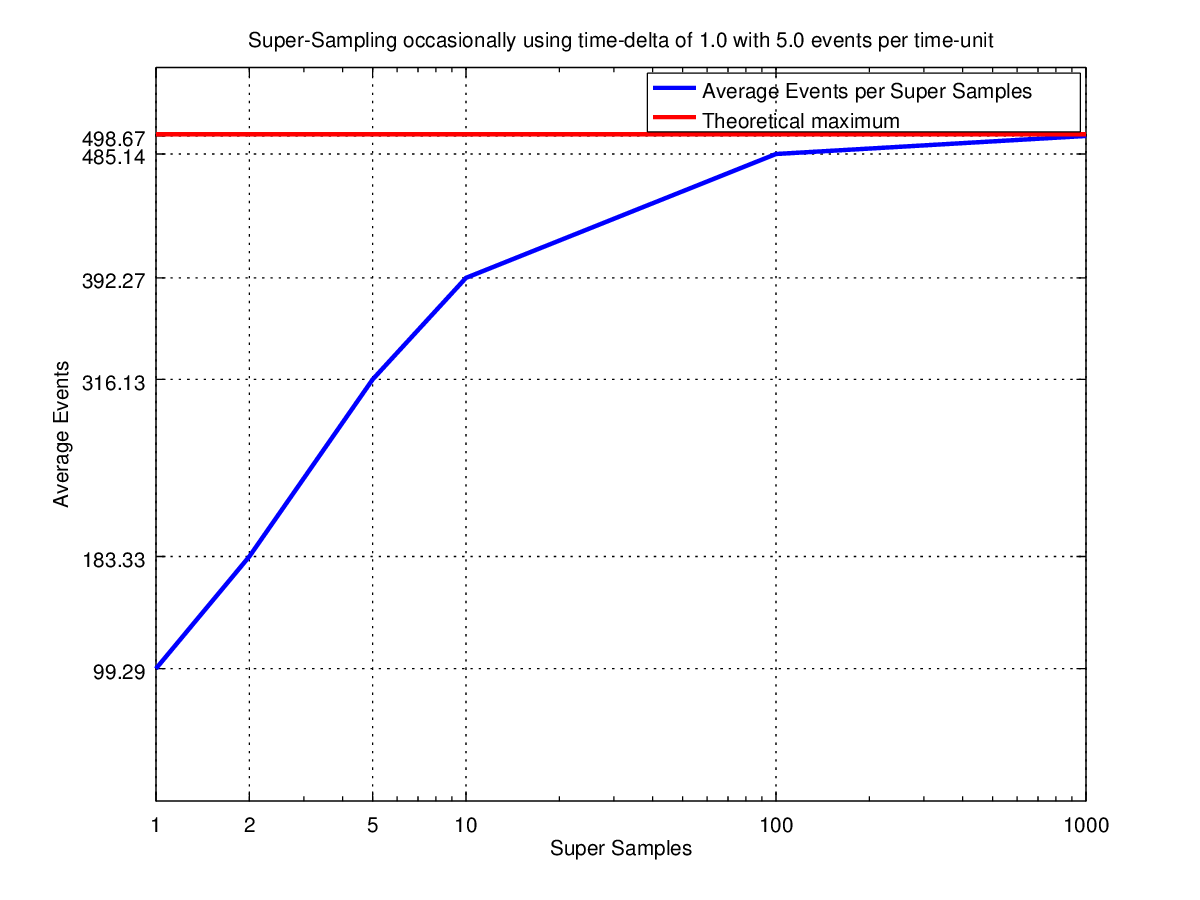
\includegraphics[width=.6\textwidth, angle=0]{./../shared/fig/samplingTest_occasionally_ss_5evts.png}
	\caption{Super-Sampling the \textit{occasional} function to visualize the influence of increasing number of super-samples on the event occurrence. Event-frequency of $\frac{1}{5}$ (average of 5 events per time-unit) with time-delta of 1, with super-samples of [1, 2, 5, 10, 100, 1000] running for 100 time-units with 100 replications. The theoretical average is 20 event within this time-frame.}
	\label{fig:sampling_occasionally_ss_5evts}
\end{figure}

\begin{figure}
	\centering
	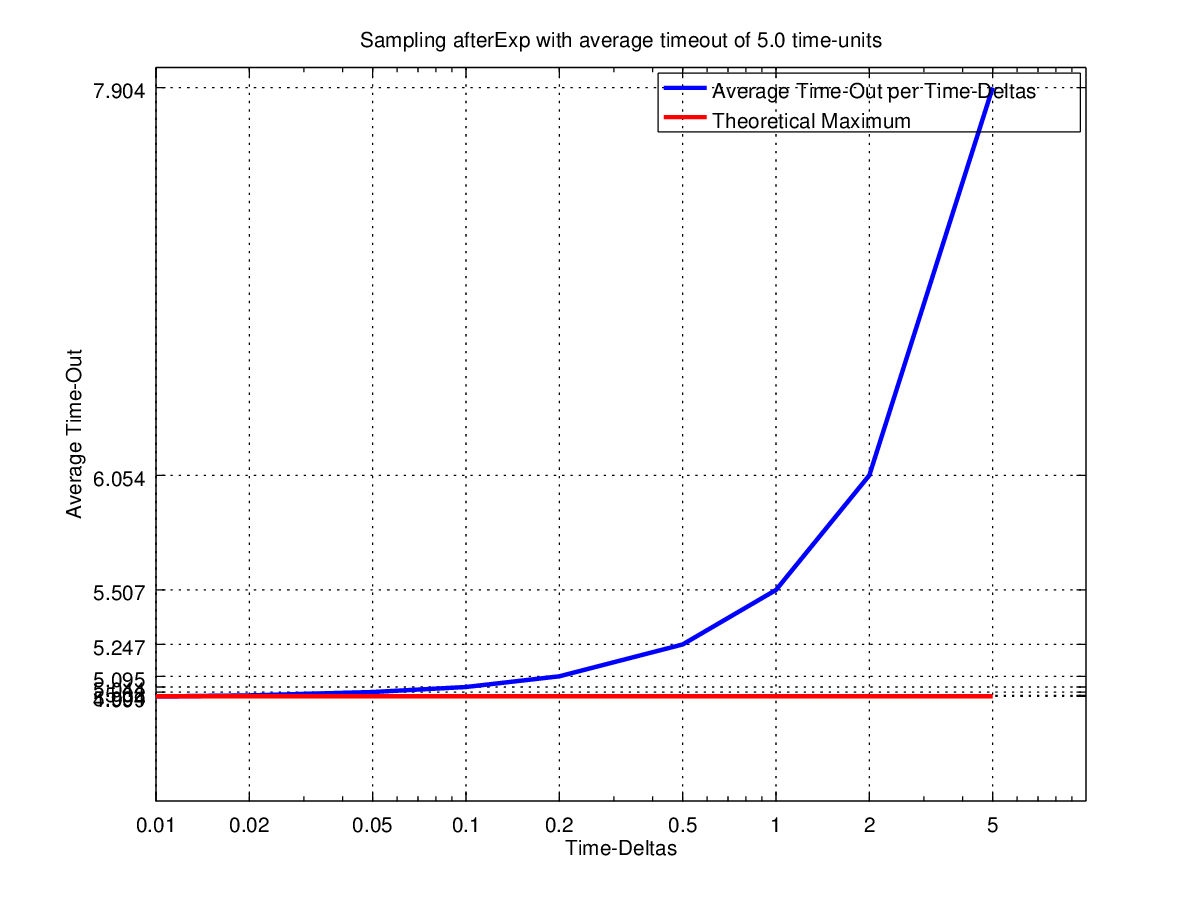
\includegraphics[width=.6\textwidth, angle=0]{./../shared/fig/samplingTest_afterExp_5time.png}
	\caption{Super-Sampling the \textit{afterExp} function to visualize the influence of increasing number of super-samples on the average time-out. Average time-out of 5 with time-delta of 1, with super-samples of [1, 2, 5, 10, 100, 1000], running 10,000 replications.}
	\label{fig:sampling_afterExp_ss_5time}
\end{figure}

\begin{figure}
	\centering
	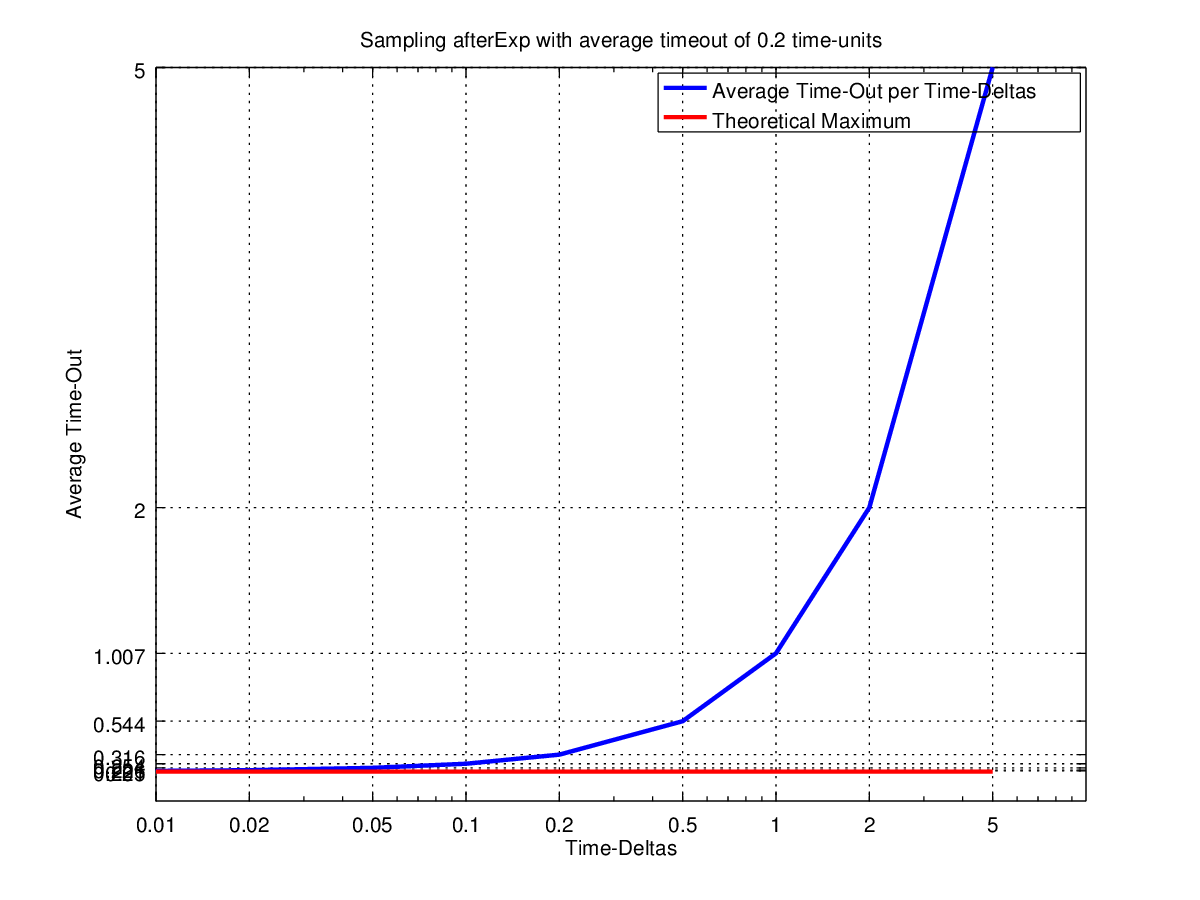
\includegraphics[width=.6\textwidth, angle=0]{./../shared/fig/samplingTest_afterExp_02time.png}
	\caption{Super-Sampling the \textit{afterExp} function to visualize the influence of increasing number of super-samples on the average time-out. Average time-out of 0.2 with time-delta of 1, with super-samples of [1, 2, 5, 10, 100, 1000], running 10,000 replications.}
	\label{fig:sampling_afterExp_ss_02time}
\end{figure}

At first this might not seem to be a real win as we still need to calculate a big number of samples every time. The big win comes though when these super-sampled signal-functions are embedded in a larger system which could run on a comparatively low frequency of e.g. 1 dt. So we are then increasing the sampling-frequency just where we need it and keep the frequency low where it is not required.

TODO: report results of using it in FrSIR ABS and discuss the *SS functions 